% Author: Izaak Neutelings (December 2020)
% Inspiration: https://tex.stackexchange.com/questions/285578/how-to-draw-parallelepiped-and-cube-with-latex/288101#288101
\documentclass[border=3pt,tikz]{standalone}
\usepackage{amsmath}\usepackage[outline]{contour} % glow around text
\usetikzlibrary{arrows,arrows.meta}
\tikzset{>=latex} % for LaTeX arrow head
\contourlength{1.5pt}

\colorlet{myblue}{blue!60!black}
\colorlet{myred}{red!80!black}
\colorlet{vcol}{green!60!black}
\tikzstyle{vvec}=[-{Latex[length=4,width=3]},thick,vcol,line cap=round]
\tikzstyle{myarr}=[-{Latex[length=3,width=2]}]
\tikzstyle{mydoublearr}=[{Latex[length=3,width=2]}-{Latex[length=3,width=2]}]

\begin{document}

% ENERGY SHELL
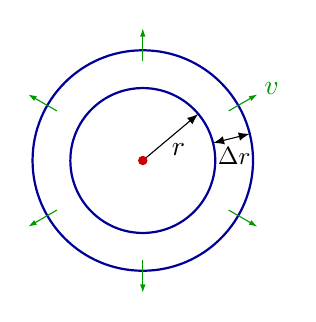
\begin{tikzpicture}
  \def\R{1.40}
  \def\r{0.92}
  \draw[myblue,thick] (0,0) circle (\r);
  \draw[myblue,thick] (0,0) circle (\R);
  \foreach \a in {30,90,...,330}{
    \draw[myarr,vcol] (\a:{0.90*\R}) -- (\a:{1.2*\R});
  }
  \node[vcol,above=2,right=-1] at (30:1.2*\R) {$v$};
  \draw[->] (0,0) -- (40:\r) node[pos=0.45,below right=-2] {$r$};
  \draw[<->] (14:\r) -- (14:\R) node[midway,right=1,below,scale=0.9] {$\Delta r$};
  \fill[myred] (0,0) circle (0.06);
  %\node[] at (120:\r) {\contour{white}{$E$}};
\end{tikzpicture}

% ENERGY AT TWO TIMES
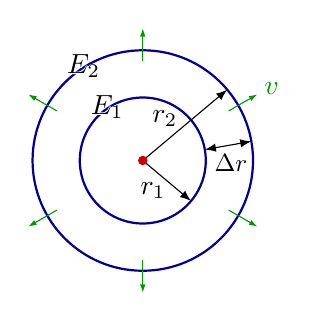
\begin{tikzpicture}
  \def\R{1.40}
  \def\r{0.80}
  \draw[myblue,thick] (0,0) circle (\r);
  \draw[myblue,thick] (0,0) circle (\R);
  \foreach \a in {30,90,...,330}{
    \draw[myarr,vcol] (\a:{0.90*\R}) -- (\a:{1.2*\R});
  }
  \node[vcol,above=2,right=-1] at (30:1.2*\R) {$v$};
  \draw[->] (0,0) -- (-40:\r) node[midway,below left=-3] {$r_1$};
  \draw[->] (0,0) -- ( 40:\R) node[pos=0.59,left=2] {$r_2$};
  \draw[<->] (10:\r) -- (10:\R) node[midway,right=1,below,scale=0.9] {$\Delta r$};
  \fill[myred] (0,0) circle (0.06);
  \node[above left=-8] at (120:\r) {\contour{white}{$E_1$}};
  \node[above left=-8] at (120:\R) {\contour{white}{$E_2$}};
\end{tikzpicture}

\end{document}